
\chapter{ZCLAIM Overview}

We introduce \zclaim, an adaptation of \xclaim to the privacy coin Zcash.
\zclaim adapts and expands on the ideas of \xclaim such as to facilitate the transfer of value from a blockchain that is not publicly auditable to a smart-contract capable blockchain supporting the required cryptographic functions.

To this end, we assume an implementation of Zcash's Sapling upgrade according to the protocol specification~\cite{hopwood2016zcash} on the issuing chain and introduce new transfer types along with their accompanying zk-SNARKs to facilitate interoperability.
These transfers fit into Zcash's shielded payment scheme and enable the issuing and redeeming of value.
Furthermore, we discuss the smart-contract logic necessary to carry out the issue and redeem protocols of \xclaim in this context.


\section{Transfers and transactions}

Along with the Spend and Output transfers of Sapling, the issuing chain offers Mint and Burn transfers.
A Mint transfer is a transfer creating value of the issued currency, i.e. increasing the circulating supply.
A Burn transfer takes the burnt amount out of circulation.
Transactions in the issuing chain may contain transparent inputs, outputs, and scripts, shielded Spend and Output transfers, and a number of either Mint or Burn transfers.

A zk-SNARK in Mint transfers proves that a shielded note has been sent to the vault on Zcash and that the minted value corresponds to the locked value.
In Burn transfers, redeemers create a note they wish to receive and encrypt it to the vault, while publishing its note commitment.
The zk-SNARK therein allows redeemers to show that the note has the correct value.
Once the vault proves that the note commitment has been added to Zcash's note commitment tree, the transaction containing the Burn transfer is included in the blockchain.

We refer to a transaction containing a Mint transfer as a \mint transaction, and one containing a Burn transfer as a \burn transaction.
Transactions may contain at most either one Mint transfer or one Burn transfer, never more.


\section{Protocols}
\label{sec:protocols_highlevel}

\zclaim define two protocols, Issue and Redeem, which are adapted from \xclaim to address the challenges described in \cref{sec:challenges}.
We present here a high-level overview of both protocols.
Diagrams for both protocols depicting the simplified sequences of steps described in this section can be seen on \cref{fig:zclaim_diagrams}.

\begin{figure}
\centering
\begin{subfigure}{.46\textwidth}
  \centering
  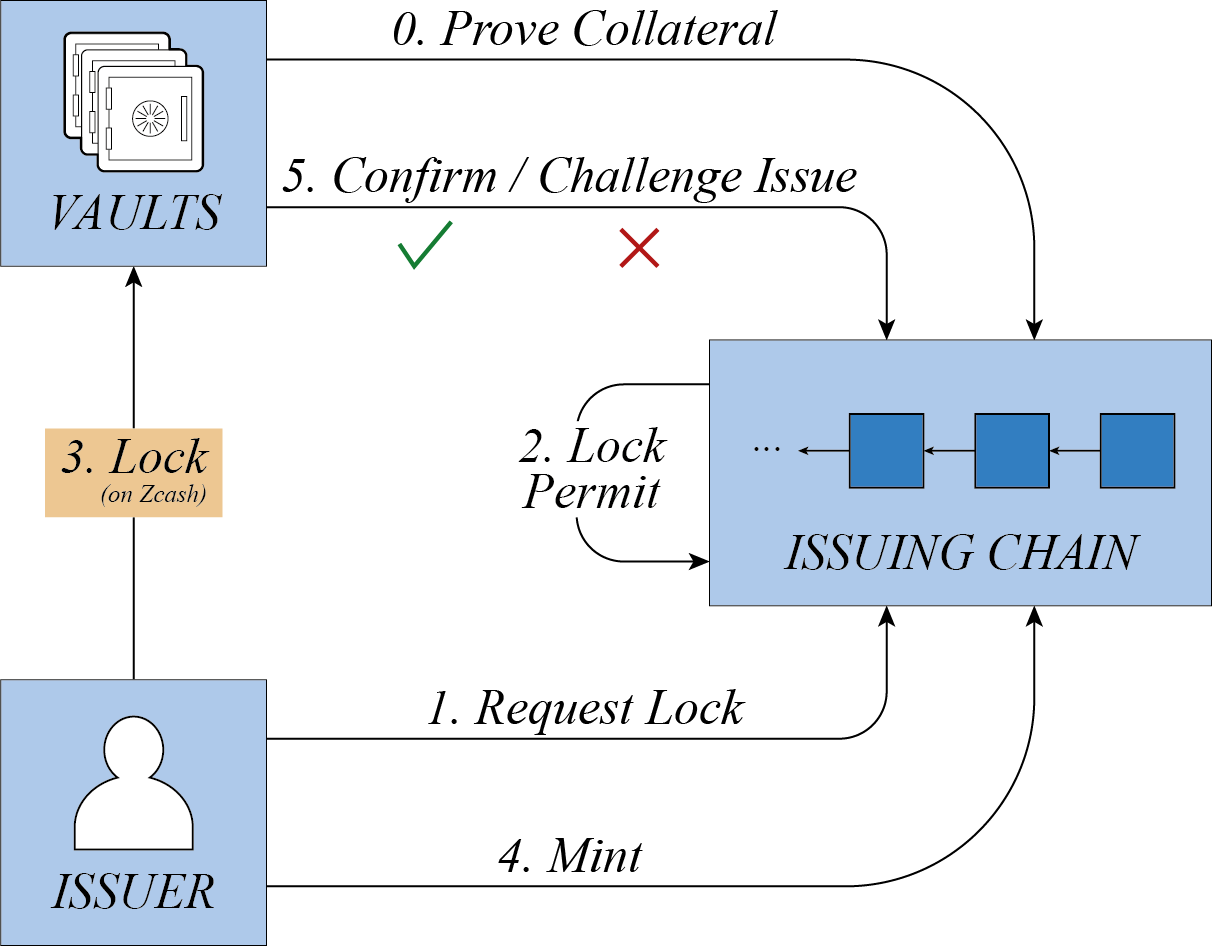
\includegraphics[width=\linewidth]{img/issue_simple.png}
  \caption{Issue}
\end{subfigure}
\quad
\begin{subfigure}{.46\textwidth}
  \centering
  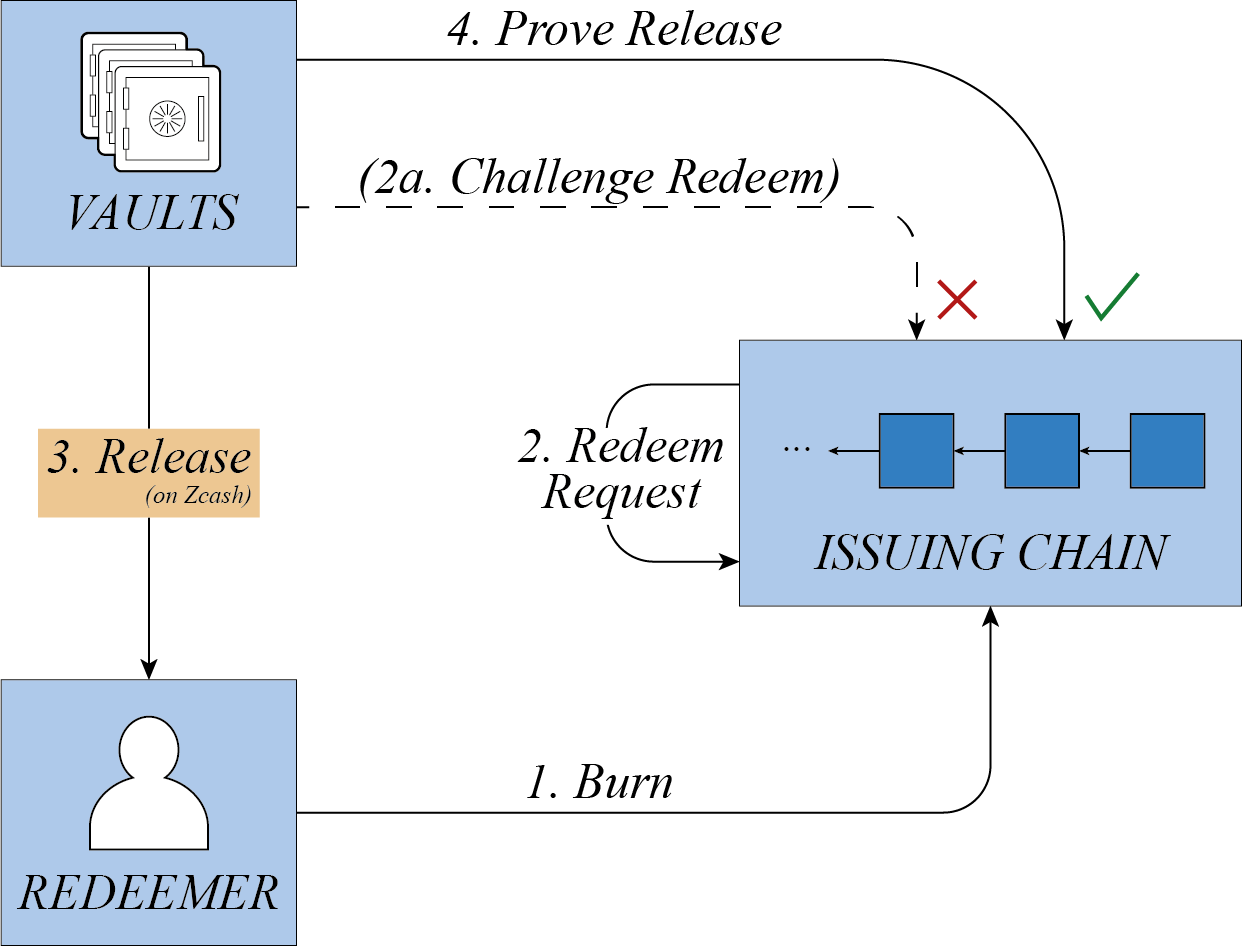
\includegraphics[width=\linewidth]{img/redeem_simple.png}
  \caption{Redeem}
\end{subfigure}
\caption{Simplified diagrams of \zclaim protocols.}
\label{fig:zclaim_diagrams}
\end{figure}

\subsection{Issuing}
\label{sec:issuing_hl}

The Issue protocol allows the creation of ICZ by locking ZEC with a vault.
It involves the following steps:

\textbf{Protocol: Issue.} Alice (issuer) locks funds with vault V on Zcash to create units of ICZ on $I$.
\begin{enumerate}
    \item \emph{Setup.} V registers with the vault registry on $I$ and locks  $ICN_{col}$ units of collateral, where it must hold that
    \begin{equation}\label{eq:collateral_issue}
        ICN_{col} \geq \vmax \cdot (1 - f) \cdot \sstd \cdot xr_{cap}
    \end{equation}
    where \vmax is the maximum amount of funds that can be locked or burned per request, $f$ is the \zclaim transaction fee and $\sstd$ is the standard collateralisation rate, all of which are defined in \cref{sec:constants}, and $xr_{cap}$ is the exchange rate at the time the vault provides a proof of capacity as explained next.
    
    In order to register as a vault, V must also provide a diversified payment address on Zcash, to which issuers will send their funds, to the vault registry.
    V further submits a \emph{proof of capacity} to the vault registry in which they prove that \cref{eq:collateral_issue} holds, hence becoming available for lock requests.
    
    \item \emph{Commit.} Alice makes a request to the issuing chain to lock her funds with vault V with diversified payment address $\dpa_\text{V}$.
    As part of this request, Alice locks a small amount of ICN \iw, her \emph{warranty collateral}, to prevent griefing attacks and compensate for V's opportunity cost in case Alice does not follow through with her request.
    
    \item \emph{Lock permit.} Subsequently, a \emph{lock permit} is created on the issuing chain granting permission to Alice to lock her funds with V.
    This permit contains a cryptographic nonce $n_{lock}$ that Alice must include in the transaction locking the funds.

    If Alice fails to execute step 4 within \dm, her warranty collateral \iw is transferred to V.
    
    \item \emph{Lock.} Alice creates a shielded transaction on Zcash, sending $ZEC_{lock}$ to V.
    Alice uses the nonce in the lock request to derive the note commitment trapdoor of the output note \n addressed to V in this transaction.
    
    \item \emph{Create.} Alice makes a request to issue $ICZ_{create}$ to a shielded address on $I$.
    To this end, Alice provides a note commitment $cm_\n$ and a Merkle proof to the root of the note commitment tree in a block header, and further proves in zero knowledge that:
    \begin{itemize}
        \item she knows a note \n with note commitment $cm_\n$, recipient $\dpa_\text{V}$ and value $ZEC_{lock}$
        \item $ICZ_{create}$ is equal to $ZEC_{lock}$ minus fees and $ZEC_{lock} \leq \vmax$
        \item the trapdoor used to generate $cm_\n$ was derived from $n_{lock}$
    \end{itemize}
    Furthermore, Alice publishes the note ciphertext $C^{\text{V}}$ of the note \n encrypted to V.
    The transaction $T_{\mintop}$ creating the funds $ICZ_{create}$ is not included in $I$ until V confirms it.
    If V fails to do so within \dci, the same amount of collateral \iw is deducted from V's collateral and transferred to Alice, and $T_{\mintop}$ is included in $I$.
    
    \item \emph{Confirm/Challenge.} V decrypts $C^{\text{V}}$ and verifies whether the resulting note has note commitment $cm_\n$.
    If this is the case, V sends a confirmation and the issuing process is complete.
    
    On the other hand, if V finds that they cannot properly decrypt $C^{\text{V}}$, they may challenge the transaction by revealing the shared secret used in the encryption.
    It can then be verified on chain that the encryption was erroneous, in which case $T_{\mintop}$ is discarded and Alice loses the funds $ZEC_{lock}$ and \iw.
\end{enumerate}

\subsection{Redeeming}
\label{sec:redeeming_hl}

The Redeem protocol allows the redeeming of ICZ for ZEC, which involves destroying or \emph{burning} ICZ on $I$ and the release of ZEC by a vault.
This is accomplished in the following sequence of steps:

\textbf{Protocol: Redeem.} Dave (redeemer) burns ICZ on $I$ and obtains ZEC from vault V.
\begin{enumerate}[start=0]
    \item \emph{Setup.} V is available to redeem, i.e.\ has not provided a \emph{proof of insolvency} to the vault registry since they last participated in an Issue procedure.
    
    \item \emph{Burn.} Dave makes a request to burn funds $ICZ_{burn}$ on $I$ by locking \iw as warranty collateral and submitting a transaction $T_{\burnop}$.
    
    \item \emph{Redeem request.} In this transaction, Dave specifies that he would like to redeem ZEC from V in a note \n with note commitment $cm_\n$, and proves in zero knowledge that:
    \begin{itemize}
        \item he knows a note \n with note commitment $cm_\n$ and value $ZEC_{release}$
        \item $ZEC_{release}$ is equal to $ICZ_{burn}$ minus fees and $ICZ_{burn} \leq \vmax$
    \end{itemize}
    
    In order to transmit the note values to V, Alice publishes the note ciphertext $C^{\text{V}}$ of the note \n encrypted to V.
    
    $T_{\burnop}$ is not included in $I$ until V confirms the release of $ZEC_{release}$.
    If V' fails to do so within \dcr, \iw is deducted from V's collateral and transferred to Dave, and $T_{\burnop}$ is discarded.
    
    \item \emph{Release.} V releases $ZEC_{release}$ to Dave by creating a note \n with note commitment $cm_\n$.

    \item \emph{Confirm/Challenge.} V waits until the relay system signals that consensus has been reached on the block in which \n was created and then submits an inclusion proof for this note.
    $T_{\burnop}$ is then included in $I$.
    
    However, if upon decryption of the note ciphertext $C^{\text{V}}$ provided by Alice in step 2, V finds that the resulting plaintext does not correspond to a note with note commitment $cm_\n$, they may challenge the transaction by revealing the shared secret used in the encryption.
    It can then be verified on chain that the encryption was erroneous, in which case $T_{\burnop}$ is discarded and Dave's warranty collateral is transferred to V.
    In this case, V does not execute step 3.
\end{enumerate}
